\chapter{Simulation: Checking the Circuit Before Loading It}
\label{ch:sim}

\section{Why You Need Simulation}

Debugging on a board is like looking for a fault blindfolded:
you can see only six LEDs, while inside there are thousands of signals, and they change
27 million times per second. That is why professionals \textbf{check the
circuit in a simulator first}---a program that computes the values of all
signals over time and draws timing diagrams.

\begin{figure}[H]
\centering
\begin{tikzpicture}
\begin{axis}[
  width=0.8\textwidth, height=5.4cm, ybar, bar width=12mm,
  symbolic x coords={Simulation, {Synthesis + routing}, {Upload to board}},
  xtick=data, ylabel={Time of one iteration, s}, ymin=0, ymax=80,
  nodes near coords, nodes near coords style={font=\sffamily\small},
  label style={font=\sffamily\small}, tick label style={font=\sffamily\small},
  axis lines*=left, grid=major, grid style={FpgaGray!20},
]
  \addplot[fill=FpgaGreen!60, draw=FpgaGreen] coordinates {(Simulation,1) ({Synthesis + routing},40) ({Upload to board},5)};
\end{axis}
\end{tikzpicture}
\caption{Typical time of one ``fix---check'' cycle for a small
project. In the simulator you can see all internal signals, while on the board you can see only the
outputs}
\end{figure}

\begin{diybox}[Simulation versus uploading]
\textbf{Task.} Check on your own project that verifying a circuit in the simulator is faster than programming the board.

\textbf{In Logra.} Open the ``27 MHz blinker'' project (the ``From an example'' card). Click ``Synthesize (Ctrl+Enter)'' and time it; then open the Waveforms tab (the ``Check'' group), set the number of cycles to 30, and run.

\textbf{Expected result.} The diagram shows all internal signals, including \code{cnt}, which you cannot see on the board; the run takes noticeably less time than the whole synthesis and upload cycle.

\textbf{How to check.} Compare your numbers with the figure above (1, 40 and 5\,s). Find a signal on the diagram that does not exist on the board pins.

\stars{1} repeat: run the diagram and find \code{cnt}. \stars{2} change: introduce a bug into the project (invert \code{led}) and find it from the diagram without going to the board. \stars{3} project: the ``Security Panel'' stage---a test scenario; acceptance criterion: a table of five events (door, night, noise, code, reset) is written, and for each one the expected state of the panel is given.
\end{diybox}

\section{The Testbench}

For simulation you write one more Verilog module---a \term{testbench}
(a ``test stand''). It has no ports: it creates the input signals itself,
connects the module under test (DUT---Device Under Test) to them, and
watches the outputs.

\begin{figure}[H]
\centering
\begin{tikzpicture}
  \node[gblock, minimum width=34mm, minimum height=20mm] (dut) {DUT\\\footnotesize module under test\\\footnotesize (gates, blink\ldots)};
  \node[block, left=18mm of dut, minimum height=20mm] (gen) {Stimulus\\generator\\\footnotesize clk, buttons};
  \node[block, right=18mm of dut, minimum height=20mm] (mon) {Checker\\\footnotesize \$display,\\\footnotesize VCD file};
  \draw[arr] (gen) -- node[above, lbl] {inputs} (dut);
  \draw[arr] (dut) -- node[above, lbl] {outputs} (mon);
  \node[draw=FpgaBlue, dashed, thick, rounded corners, fit=(gen)(dut)(mon), inner sep=4mm, label={[font=\sffamily\small\bfseries, text=FpgaBlue]above:module tb (testbench)}] {};
\end{tikzpicture}
\caption{Structure of a testbench}
\end{figure}

A testbench may use constructs that \emph{cannot} be synthesized into
hardware but are handy for modeling:
\begin{itemize}
  \item \code{\#10;}---wait for 10 time units;
  \item \code{initial begin ... end}---perform actions once at the start
        of the simulation;
  \item \code{\$display(...)}, \code{\$monitor(...)}---print to the console;
  \item \code{\$dumpfile}, \code{\$dumpvars}---write all signals to a
        \code{.vcd} file for viewing in GTKWave;
  \item \code{\$finish}---end the simulation.
\end{itemize}

Because of this, files named \code{tb\_*.v} are not meant for the \emph{Code}
tab of Logra as the top module: its synthesizer rejects \code{\$finish} and
delays, and no RTL appears. Run a testbench with \code{iverilog} and
\code{vvp} in a terminal; in Logra, use the \emph{Waveforms} tab, which builds
a testbench around your module on its own.

\begin{diybox}[A testbench without Verilog: Logra scenarios]
\textbf{Task.} Compare the testbench from the book with what the Waveforms tab does: it creates a testbench around your module by itself and applies the given signals to the inputs.

\textbf{In Logra.} Open the ``Logic gates'' project (\code{gates.v}), Waveforms tab. The ``Sweep inputs'' scenario replaces the loop with \code{\#10;} from \code{tb\_gates.v}. Also add an ``Events'' section and apply your own pulses to \code{a} and \code{b}.

\textbf{Expected result.} Two inputs give four combinations; the outputs show the same values as in the table of project~1.

\textbf{How to check.} Select the signals \code{a}, \code{b}, \code{led}, and compare the rows with Table~\ref{tab:gates}. Optional step: in a terminal run \code{iverilog} and \code{vvp} as shown below and compare the output.

\stars{1} repeat: a full sweep of the inputs of project~1. \stars{2} change: apply the same sequence by hand through ``Events'' and make sure the picture is the same. \stars{3} project: the ``Security Panel'' stage---checking the combinational part; acceptance criterion: sweeping all $2^3$ combinations of the sensors gives a table that matches the ``2 out of 3'' voting formula.
\end{diybox}

\section{Example 1: The Truth Table of Project 1}

\vfile{\codepath/01_gates/tb_gates.v}{code/01\_gates/tb\_gates.v}

Running in the terminal:
\begin{vcode}[bash]
iverilog -o tb_gates tb_gates.v gates.v   # compile
vvp tb_gates                              # simulate
\end{vcode}

The result (this is real simulator output):
\begin{vcode}[text]
 a b | AND OR NOT NAND NOR XOR
 0 0 |  0   0   1    1    1   0
 1 0 |  0   1   0    1    0   1
 0 1 |  0   1   1    1    0   1
 1 1 |  1   1   0    0    0   0
\end{vcode}

Compare it with Table~\ref{tab:gates_all} in Chapter~\ref{ch:gates}---everything matches.

\begin{diybox}[The truth table of project 1]
\textbf{Task.} Obtain the truth table of the six functions and compare it with Table~\ref{tab:gates_all} in Chapter~\ref{ch:gates}.

\textbf{In Logra.} The ``Logic gates'' project, Waveforms tab: ``Sweep inputs'', signals \code{a}, \code{b} and all the outputs.

\textbf{Expected result.} For $a=b=1$ only AND and OR equal 1; for $a=b=0$ NOT, NAND and NOR equal 1; XOR equals 1 only when the inputs differ.

\textbf{How to check.} Build the table by hand from the diagram and compare it with the simulator output from the book: the order of rows in Logra may differ, but the set of values is the same.

\stars{1} repeat: fill in the table of six columns. \stars{2} find the bug: in \code{gates.v} change \code{\textasciicircum} to \code{|} and show in which row of the diagram XOR became wrong. \stars{3} project: a sweep for the function \code{alarm = door \& (night | armed)}; acceptance criterion: the eight rows match the truth table from the chapter on logic gates.
\end{diybox}

\section{Example 2: A Blinker with a Reduced Frequency}

Checking a blinker at the real frequency takes too long: to wait for a single
toggle you would have to simulate $13.5$ million clock cycles. That is why in the
\code{blink} module the frequency is made a \code{parameter}, and the testbench sets
\code{CLK\_HZ = 20}: the LED toggles every 10 clock cycles.

\vfile{\codepath/02_blink/tb_blink.v}{code/02\_blink/tb\_blink.v}

A fragment of the output:
\begin{vcode}[text]
t =    0.0 ns  cnt =  0  led = 111111
t =   18.5 ns  cnt =  1  led = 111111
...
t =  314.5 ns  cnt =  9  led = 111111
t =  351.5 ns  cnt =  0  led = 000000
t =  388.5 ns  cnt =  1  led = 000000
\end{vcode}

After \code{cnt = 9} (that is \code{HALF - 1}) the counter resets, and the
LEDs light up (\code{000000}). The circuit works as intended.

\begin{diybox}[A blinker with a reduced frequency]
\textbf{Task.} Check that the blinker LED toggles every 10 clock cycles when \code{CLK\_HZ = 20}, and find the parameter for which it toggles every 4 clock cycles.

\textbf{In Logra.} The ``27 MHz blinker'' project: in the Code tab replace the \code{CLK\_HZ} parameter with 20, then open the Waveforms tab and set the number of cycles to 25.

\textbf{Expected result.} \code{cnt} counts $0\ldots9$, resets at the value 9, and at that moment \code{led} changes from \code{111111} to \code{000000}; to toggle every 4 clock cycles you need \code{CLK\_HZ = 8}.

\textbf{How to check.} Waveforms, signals \code{cnt} and \code{led}; use the cursor to measure the distance between two toggles.

\stars{1} repeat: a toggle period of 10 clock cycles. \stars{2} change: the parameter \code{CLK\_HZ = 8} and a recalculation. \stars{3} project: the ``Security Panel'' stage---a speeded-up model; acceptance criterion: the beep counter is reduced so that the siren toggles within 8 clock cycles, and the diagram shows both the tone and the pause.
\end{diybox}

\section{Timing Diagrams in GTKWave}

The command \code{gtkwave tb\_blink.vcd} opens a window that looks like
Fig.~\ref{fig:gtkwave}. On the left you pick signals; on the right you see their diagrams.

\begin{figure}[H]
\centering
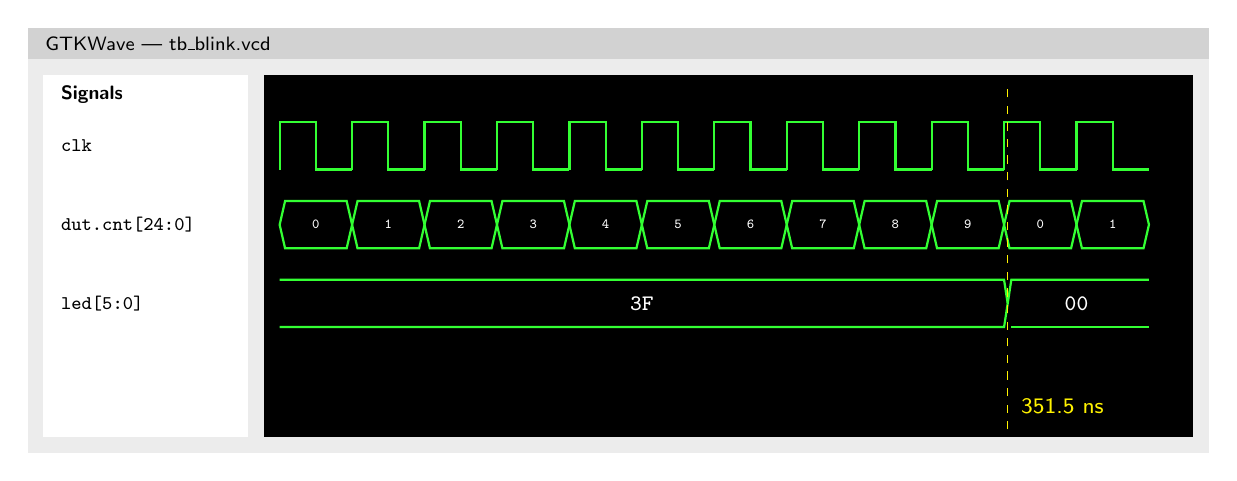
\begin{tikzpicture}
  \fill[gray!15] (0,0) rectangle (15,5.4);
  \fill[gray!35] (0,5.0) rectangle (15,5.4);
  \node[font=\sffamily\scriptsize, anchor=west] at (0.1,5.2) {GTKWave --- tb\_blink.vcd};
  \fill[white] (0.2,0.2) rectangle (2.8,4.8);
  \node[font=\sffamily\scriptsize\bfseries, anchor=west] at (0.3,4.55) {Signals};
  \foreach \n/\y in {clk/3.9, dut.cnt[24:0]/2.9, led[5:0]/1.9} \node[font=\ttfamily\scriptsize, anchor=west] at (0.3,\y) {\n};
  \fill[black] (3.0,0.2) rectangle (14.8,4.8);
  \begin{scope}[shift={(3.2,0)}, x=0.46cm]
    \foreach \i in {0,...,11} {
      \draw[green!80!white, thick] (\i*2,3.6) -- (\i*2,4.2) -- (\i*2+1,4.2) -- (\i*2+1,3.6) -- (\i*2+2,3.6);
    }
    \foreach \i/\v in {0/0,1/1,2/2,3/3,4/4,5/5,6/6,7/7,8/8,9/9,10/0,11/1} {
      \draw[green!80!white, thick] (\i*2+0.15,2.6) -- (\i*2+1.85,2.6) -- (\i*2+2,2.9) -- (\i*2+1.85,3.2) -- (\i*2+0.15,3.2) -- (\i*2,2.9) -- cycle;
      \node[white, font=\ttfamily\tiny] at (\i*2+1,2.9) {\v};
    }
    \draw[green!80!white, thick] (0,1.6) -- (20,1.6) -- (20.1,1.9) -- (20,2.2) -- (0,2.2);
    \node[white, font=\ttfamily\footnotesize] at (10,1.9) {3F};
    \draw[green!80!white, thick] (20.1,1.9) -- (20.2,2.2) -- (24,2.2); \draw[green!80!white, thick] (20.2,1.6) -- (24,1.6);
    \node[white, font=\ttfamily\footnotesize] at (22,1.9) {00};
    \draw[yellow, dashed] (20.1,0.3) -- (20.1,4.7);
    \node[yellow, font=\sffamily\footnotesize, anchor=west] at (20.2,0.6) {351.5 ns};
  \end{scope}
\end{tikzpicture}
\caption{This is what the simulation result looks like in GTKWave (schematic)}
\label{fig:gtkwave}
\end{figure}

\begin{warnbox}[Simulation does not replace the board]
The simulator checks the \emph{logic}, but it knows nothing about button bounce, delays
in wires, or mistakes in the \code{.cst} file. That is why the last step is always
a check on a real board.
\end{warnbox}

\begin{diybox}[Reading a diagram like an engineer]
\textbf{Task.} Learn to use the diagram: choosing signals, the HEX format, the cursor for measuring time.

\textbf{In Logra.} The Waveforms tab on the ``27 MHz blinker'' project (or on \code{counter4.v} from Chapter~\ref{ch:bridge}). Select \code{clk}, \code{cnt}, \code{led}; display the bus in HEX format (values like \code{0x..}).

\textbf{Expected result.} Bus values are read as a whole rather than bit by bit; with the cursor you measure the period of \code{clk} and the interval between two toggles of \code{led}.

\textbf{How to check.} Compare the result with Fig.~\ref{fig:gtkwave}: the set of signals and the order of rows are the same as in GTKWave.

\stars{1} repeat: find on the diagram at which clock cycle \code{cnt} resets. \stars{2} change: add an internal signal to the list and find its value at the 7th clock cycle. \stars{3} project: the ``Security Panel'' stage---a verification report; acceptance criterion: a set of signals (state, sensors, siren) is saved, from which any scenario is easy to check.
\end{diybox}
